\documentclass[a4paper, oneside, final]{memoir}
\usepackage[T1]{fontenc}
\usepackage[utf8]{inputenc}
\usepackage[british]{babel}
\usepackage{amsmath}
\usepackage{amsthm}
\usepackage{ifthen}
\usepackage{verbatim}

% bedre orddeling Gør at der som minimum skal blive to tegn på linien ved
% orddeling og minimum flyttes to tegn ned på næste linie. Desværre er værdien
% anvendt af babel »12«, hvilket kan give orddelingen »h-vor«.
\renewcommand{\britishhyphenmins}{22} 

% Fix of fancyref to work with memoir. Makes references look
% nice. Redefines memoir \fref and \Fref to \refer and \Refer.
% \usepackage{refer}             %
% As we dont really have any use for \fref and \Fref we just undefine what
% memoir defined them as, so fancyref can define what it wants.
\let\fref\undefined
\let\Fref\undefined
\usepackage{fancyref} % Better reference. 

\usepackage{pdflscape} % Gør landscape-environmentet tilgængeligt
\usepackage{fixme}     % Indsæt "fixme" noter i drafts.
\usepackage{hyperref}  % Indsæter links (interne og eksterne) i PDF

\usepackage[format=hang]{caption,subfig}
\usepackage{graphicx}
\usepackage{color}
\usepackage{stmaryrd}
\usepackage{amssymb}
\usepackage{listings}
\usepackage{ulem} % \sout - strike-through
\usepackage{tikz}

%\renewcommand{\ttdefault}{txtt} % Bedre typewriter font
% \usepackage[sc]{mathpazo}     % Palatino font
%\renewcommand{\rmdefault}{urw-garamond} % Garamond
%\usepackage[urw-garamond]{mathdesign}

% \overfullrule=5pt
% \setsecnumdepth{part}
\setcounter{secnumdepth}{1} % Sæt overskriftsnummereringsdybde. Disable = -1.
\setlength{\parskip}{0.25in}

\title{Statistical Methods for Machine Learning\\Case 1}

\author{Troels Henriksen (athas@sigkill.dk) \\ Daniel Fairchild
  (daniel.fairchild@gmail.com)}

\date{\today}
\pagestyle{plain}

\newcommand{\nfrac}[2]{\frac{\displaystyle{#1}}{\displaystyle{#2}}}

\begin{document}

\maketitle

We have never used R before, so for the novelty, that is the language
we have decided to use for much of the assignment.

\section*{Question 1.1}

\begin{figure}
 \begin{centering}
    % GNUPLOT: LaTeX picture with Postscript
\begingroup
  \makeatletter
  \providecommand\color[2][]{%
    \GenericError{(gnuplot) \space\space\space\@spaces}{%
      Package color not loaded in conjunction with
      terminal option `colourtext'%
    }{See the gnuplot documentation for explanation.%
    }{Either use 'blacktext' in gnuplot or load the package
      color.sty in LaTeX.}%
    \renewcommand\color[2][]{}%
  }%
  \providecommand\includegraphics[2][]{%
    \GenericError{(gnuplot) \space\space\space\@spaces}{%
      Package graphicx or graphics not loaded%
    }{See the gnuplot documentation for explanation.%
    }{The gnuplot epslatex terminal needs graphicx.sty or graphics.sty.}%
    \renewcommand\includegraphics[2][]{}%
  }%
  \providecommand\rotatebox[2]{#2}%
  \@ifundefined{ifGPcolor}{%
    \newif\ifGPcolor
    \GPcolortrue
  }{}%
  \@ifundefined{ifGPblacktext}{%
    \newif\ifGPblacktext
    \GPblacktextfalse
  }{}%
  % define a \g@addto@macro without @ in the name:
  \let\gplgaddtomacro\g@addto@macro
  % define empty templates for all commands taking text:
  \gdef\gplbacktext{}%
  \gdef\gplfronttext{}%
  \makeatother
  \ifGPblacktext
    % no textcolor at all
    \def\colorrgb#1{}%
    \def\colorgray#1{}%
  \else
    % gray or color?
    \ifGPcolor
      \def\colorrgb#1{\color[rgb]{#1}}%
      \def\colorgray#1{\color[gray]{#1}}%
      \expandafter\def\csname LTw\endcsname{\color{white}}%
      \expandafter\def\csname LTb\endcsname{\color{black}}%
      \expandafter\def\csname LTa\endcsname{\color{black}}%
      \expandafter\def\csname LT0\endcsname{\color[rgb]{1,0,0}}%
      \expandafter\def\csname LT1\endcsname{\color[rgb]{0,1,0}}%
      \expandafter\def\csname LT2\endcsname{\color[rgb]{0,0,1}}%
      \expandafter\def\csname LT3\endcsname{\color[rgb]{1,0,1}}%
      \expandafter\def\csname LT4\endcsname{\color[rgb]{0,1,1}}%
      \expandafter\def\csname LT5\endcsname{\color[rgb]{1,1,0}}%
      \expandafter\def\csname LT6\endcsname{\color[rgb]{0,0,0}}%
      \expandafter\def\csname LT7\endcsname{\color[rgb]{1,0.3,0}}%
      \expandafter\def\csname LT8\endcsname{\color[rgb]{0.5,0.5,0.5}}%
    \else
      % gray
      \def\colorrgb#1{\color{black}}%
      \def\colorgray#1{\color[gray]{#1}}%
      \expandafter\def\csname LTw\endcsname{\color{white}}%
      \expandafter\def\csname LTb\endcsname{\color{black}}%
      \expandafter\def\csname LTa\endcsname{\color{black}}%
      \expandafter\def\csname LT0\endcsname{\color{black}}%
      \expandafter\def\csname LT1\endcsname{\color{black}}%
      \expandafter\def\csname LT2\endcsname{\color{black}}%
      \expandafter\def\csname LT3\endcsname{\color{black}}%
      \expandafter\def\csname LT4\endcsname{\color{black}}%
      \expandafter\def\csname LT5\endcsname{\color{black}}%
      \expandafter\def\csname LT6\endcsname{\color{black}}%
      \expandafter\def\csname LT7\endcsname{\color{black}}%
      \expandafter\def\csname LT8\endcsname{\color{black}}%
    \fi
  \fi
  \setlength{\unitlength}{0.0500bp}%
  \begin{picture}(7200.00,5040.00)%
    \gplgaddtomacro\gplbacktext{%
      \csname LTb\endcsname%
      \put(1078,704){\makebox(0,0)[r]{\strut{} 0}}%
      \put(1078,1168){\makebox(0,0)[r]{\strut{} 0.05}}%
      \put(1078,1632){\makebox(0,0)[r]{\strut{} 0.1}}%
      \put(1078,2096){\makebox(0,0)[r]{\strut{} 0.15}}%
      \put(1078,2559){\makebox(0,0)[r]{\strut{} 0.2}}%
      \put(1078,3023){\makebox(0,0)[r]{\strut{} 0.25}}%
      \put(1078,3487){\makebox(0,0)[r]{\strut{} 0.3}}%
      \put(1078,3951){\makebox(0,0)[r]{\strut{} 0.35}}%
      \put(1078,4415){\makebox(0,0)[r]{\strut{} 0.4}}%
      \put(2089,484){\makebox(0,0){\strut{}-5}}%
      \put(3246,484){\makebox(0,0){\strut{} 0}}%
      \put(4402,484){\makebox(0,0){\strut{} 5}}%
      \put(5559,484){\makebox(0,0){\strut{} 10}}%
      \put(6715,484){\makebox(0,0){\strut{} 15}}%
      \put(176,2739){\rotatebox{-270}{\makebox(0,0){\strut{}Y}}}%
      \put(4006,154){\makebox(0,0){\strut{}X}}%
    }%
    \gplgaddtomacro\gplfronttext{%
      \csname LTb\endcsname%
      \put(5816,4602){\makebox(0,0)[r]{\strut{}$\mu$=-1, $\sigma$=1}}%
      \csname LTb\endcsname%
      \put(5816,4382){\makebox(0,0)[r]{\strut{}$\mu$=2, $\sigma$=2}}%
      \csname LTb\endcsname%
      \put(5816,4162){\makebox(0,0)[r]{\strut{}$\mu$=3, $\sigma$=3}}%
    }%
    \gplbacktext
    \put(0,0){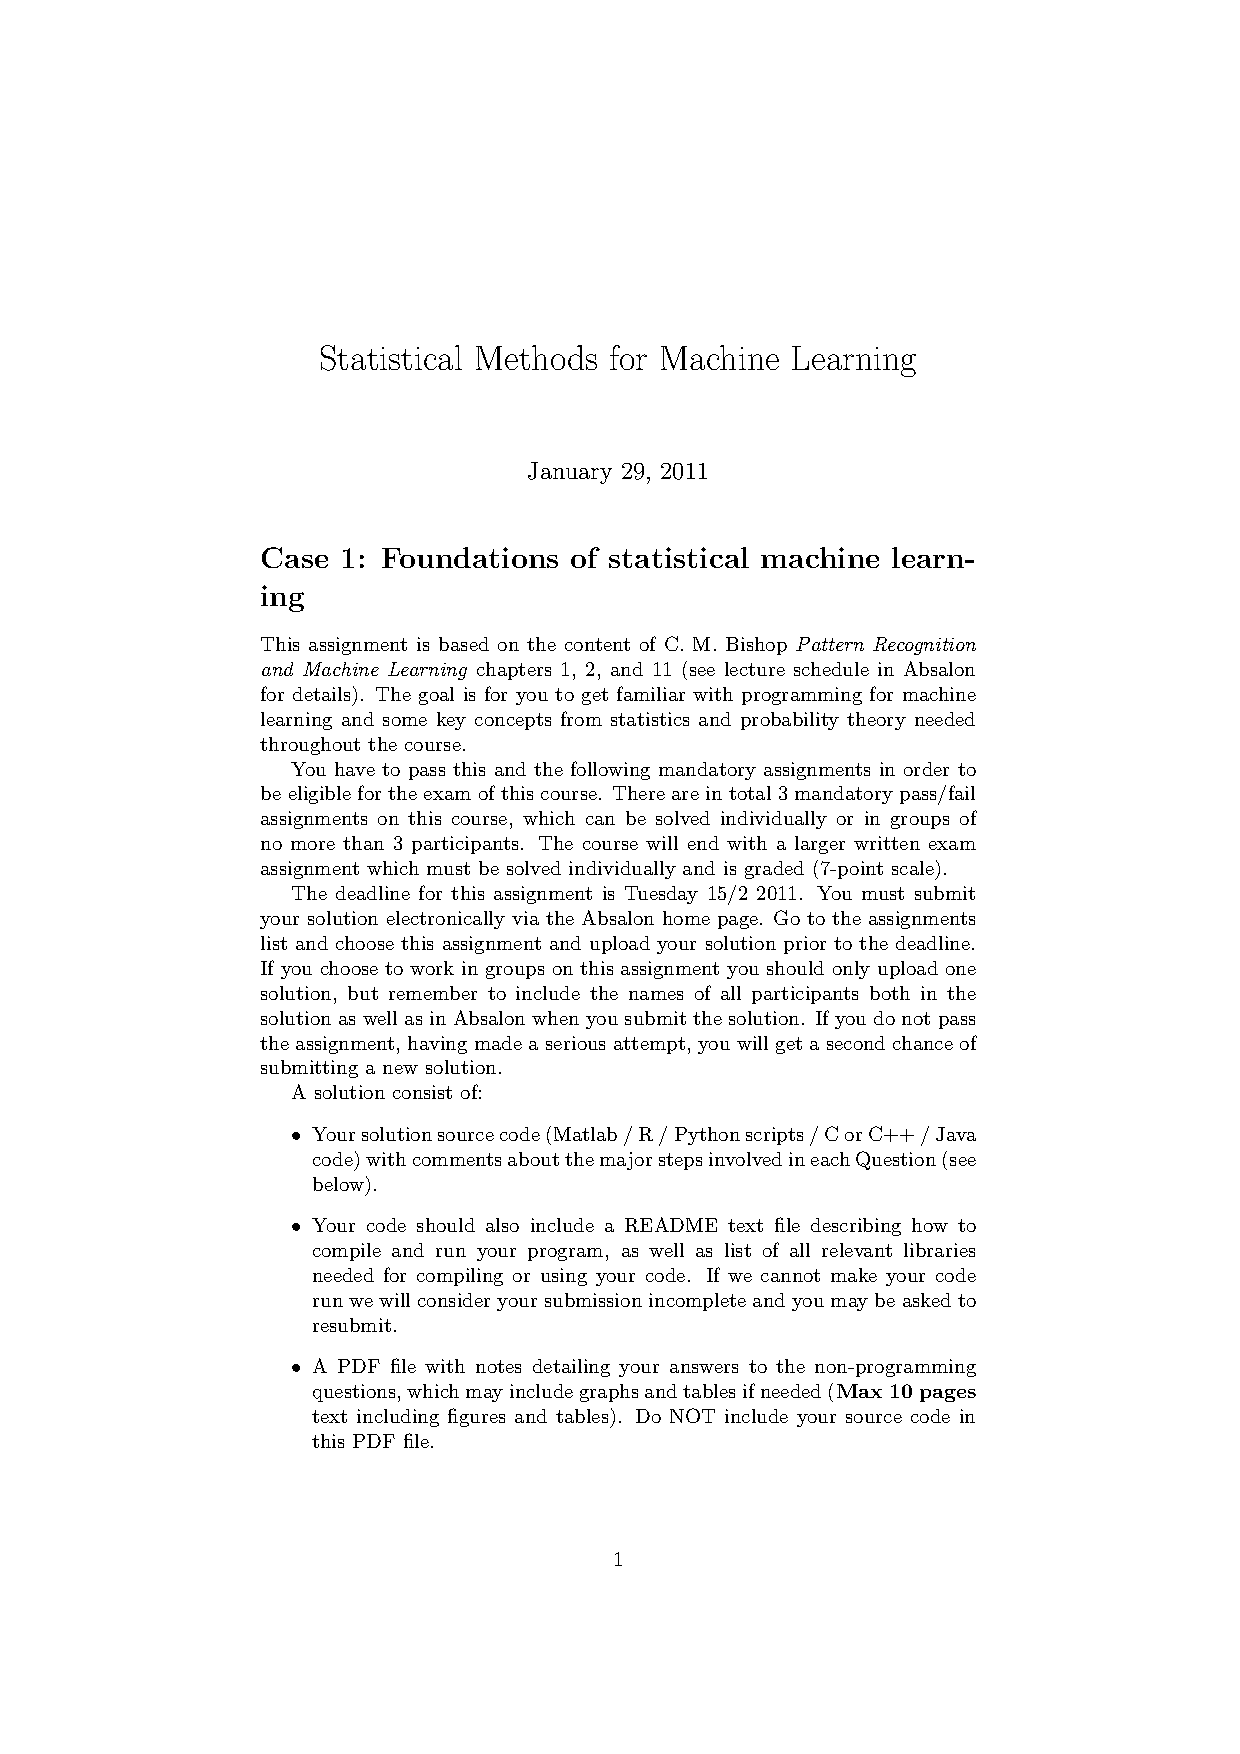
\includegraphics{tex_out/case1}}%
    \gplfronttext
  \end{picture}%
\endgroup

  \label{foobar}
 \end{centering}
\end{figure}

\subsection{hmmm...}
The following plot has been produced through straightforward use of
the \texttt{dnorm} function and plotting facilities in R.  A thousand
sample points have been used.  The code for this question is in the
file \texttt{question11.R}.



\section*{Question 1.3}
\begin{figure}
 \begin{centering}
    % GNUPLOT: LaTeX picture with Postscript
\begingroup
  \makeatletter
  \providecommand\color[2][]{%
    \GenericError{(gnuplot) \space\space\space\@spaces}{%
      Package color not loaded in conjunction with
      terminal option `colourtext'%
    }{See the gnuplot documentation for explanation.%
    }{Either use 'blacktext' in gnuplot or load the package
      color.sty in LaTeX.}%
    \renewcommand\color[2][]{}%
  }%
  \providecommand\includegraphics[2][]{%
    \GenericError{(gnuplot) \space\space\space\@spaces}{%
      Package graphicx or graphics not loaded%
    }{See the gnuplot documentation for explanation.%
    }{The gnuplot epslatex terminal needs graphicx.sty or graphics.sty.}%
    \renewcommand\includegraphics[2][]{}%
  }%
  \providecommand\rotatebox[2]{#2}%
  \@ifundefined{ifGPcolor}{%
    \newif\ifGPcolor
    \GPcolortrue
  }{}%
  \@ifundefined{ifGPblacktext}{%
    \newif\ifGPblacktext
    \GPblacktextfalse
  }{}%
  % define a \g@addto@macro without @ in the name:
  \let\gplgaddtomacro\g@addto@macro
  % define empty templates for all commands taking text:
  \gdef\gplbacktext{}%
  \gdef\gplfronttext{}%
  \makeatother
  \ifGPblacktext
    % no textcolor at all
    \def\colorrgb#1{}%
    \def\colorgray#1{}%
  \else
    % gray or color?
    \ifGPcolor
      \def\colorrgb#1{\color[rgb]{#1}}%
      \def\colorgray#1{\color[gray]{#1}}%
      \expandafter\def\csname LTw\endcsname{\color{white}}%
      \expandafter\def\csname LTb\endcsname{\color{black}}%
      \expandafter\def\csname LTa\endcsname{\color{black}}%
      \expandafter\def\csname LT0\endcsname{\color[rgb]{1,0,0}}%
      \expandafter\def\csname LT1\endcsname{\color[rgb]{0,1,0}}%
      \expandafter\def\csname LT2\endcsname{\color[rgb]{0,0,1}}%
      \expandafter\def\csname LT3\endcsname{\color[rgb]{1,0,1}}%
      \expandafter\def\csname LT4\endcsname{\color[rgb]{0,1,1}}%
      \expandafter\def\csname LT5\endcsname{\color[rgb]{1,1,0}}%
      \expandafter\def\csname LT6\endcsname{\color[rgb]{0,0,0}}%
      \expandafter\def\csname LT7\endcsname{\color[rgb]{1,0.3,0}}%
      \expandafter\def\csname LT8\endcsname{\color[rgb]{0.5,0.5,0.5}}%
    \else
      % gray
      \def\colorrgb#1{\color{black}}%
      \def\colorgray#1{\color[gray]{#1}}%
      \expandafter\def\csname LTw\endcsname{\color{white}}%
      \expandafter\def\csname LTb\endcsname{\color{black}}%
      \expandafter\def\csname LTa\endcsname{\color{black}}%
      \expandafter\def\csname LT0\endcsname{\color{black}}%
      \expandafter\def\csname LT1\endcsname{\color{black}}%
      \expandafter\def\csname LT2\endcsname{\color{black}}%
      \expandafter\def\csname LT3\endcsname{\color{black}}%
      \expandafter\def\csname LT4\endcsname{\color{black}}%
      \expandafter\def\csname LT5\endcsname{\color{black}}%
      \expandafter\def\csname LT6\endcsname{\color{black}}%
      \expandafter\def\csname LT7\endcsname{\color{black}}%
      \expandafter\def\csname LT8\endcsname{\color{black}}%
    \fi
  \fi
  \setlength{\unitlength}{0.0500bp}%
  \begin{picture}(7200.00,5040.00)%
    \gplgaddtomacro\gplbacktext{%
      \csname LTb\endcsname%
      \put(682,704){\makebox(0,0)[r]{\strut{}-1}}%
      \put(682,1518){\makebox(0,0)[r]{\strut{} 0}}%
      \put(682,2332){\makebox(0,0)[r]{\strut{} 1}}%
      \put(682,3147){\makebox(0,0)[r]{\strut{} 2}}%
      \put(682,3961){\makebox(0,0)[r]{\strut{} 3}}%
      \put(682,4775){\makebox(0,0)[r]{\strut{} 4}}%
      \put(814,484){\makebox(0,0){\strut{}-1}}%
      \put(1563,484){\makebox(0,0){\strut{}-0.5}}%
      \put(2311,484){\makebox(0,0){\strut{} 0}}%
      \put(3060,484){\makebox(0,0){\strut{} 0.5}}%
      \put(3809,484){\makebox(0,0){\strut{} 1}}%
      \put(4557,484){\makebox(0,0){\strut{} 1.5}}%
      \put(5306,484){\makebox(0,0){\strut{} 2}}%
      \put(6054,484){\makebox(0,0){\strut{} 2.5}}%
      \put(6803,484){\makebox(0,0){\strut{} 3}}%
      \put(176,2739){\rotatebox{-270}{\makebox(0,0){\strut{}Y}}}%
      \put(3808,154){\makebox(0,0){\strut{}X}}%
    }%
    \gplgaddtomacro\gplfronttext{%
      \csname LTb\endcsname%
      \put(5816,4602){\makebox(0,0)[r]{\strut{}Generated $\sigma$=1 $\mu=(1,1)^T$}}%
      \csname LTb\endcsname%
      \put(5816,4382){\makebox(0,0)[r]{\strut{}Actual $\mu$}}%
      \csname LTb\endcsname%
      \put(5816,4162){\makebox(0,0)[r]{\strut{}Sampled  $\mu$}}%
    }%
    \gplbacktext
    \put(0,0){\includegraphics{tex_out/case3}}%
    \gplfronttext
  \end{picture}%
\endgroup

  \label{foobar}
 \end{centering}
\end{figure}

The following plot has been produced through straightforward use of
the \texttt{dnorm} function and plotting facilities in R.  A thousand
sample points have been used.  The code for this question is in the
file \texttt{question11.R}.


\section*{Question 1.9}
\begin{figure}
 \begin{centering}
    % GNUPLOT: LaTeX picture with Postscript
\begingroup
  \makeatletter
  \providecommand\color[2][]{%
    \GenericError{(gnuplot) \space\space\space\@spaces}{%
      Package color not loaded in conjunction with
      terminal option `colourtext'%
    }{See the gnuplot documentation for explanation.%
    }{Either use 'blacktext' in gnuplot or load the package
      color.sty in LaTeX.}%
    \renewcommand\color[2][]{}%
  }%
  \providecommand\includegraphics[2][]{%
    \GenericError{(gnuplot) \space\space\space\@spaces}{%
      Package graphicx or graphics not loaded%
    }{See the gnuplot documentation for explanation.%
    }{The gnuplot epslatex terminal needs graphicx.sty or graphics.sty.}%
    \renewcommand\includegraphics[2][]{}%
  }%
  \providecommand\rotatebox[2]{#2}%
  \@ifundefined{ifGPcolor}{%
    \newif\ifGPcolor
    \GPcolortrue
  }{}%
  \@ifundefined{ifGPblacktext}{%
    \newif\ifGPblacktext
    \GPblacktextfalse
  }{}%
  % define a \g@addto@macro without @ in the name:
  \let\gplgaddtomacro\g@addto@macro
  % define empty templates for all commands taking text:
  \gdef\gplbacktext{}%
  \gdef\gplfronttext{}%
  \makeatother
  \ifGPblacktext
    % no textcolor at all
    \def\colorrgb#1{}%
    \def\colorgray#1{}%
  \else
    % gray or color?
    \ifGPcolor
      \def\colorrgb#1{\color[rgb]{#1}}%
      \def\colorgray#1{\color[gray]{#1}}%
      \expandafter\def\csname LTw\endcsname{\color{white}}%
      \expandafter\def\csname LTb\endcsname{\color{black}}%
      \expandafter\def\csname LTa\endcsname{\color{black}}%
      \expandafter\def\csname LT0\endcsname{\color[rgb]{1,0,0}}%
      \expandafter\def\csname LT1\endcsname{\color[rgb]{0,1,0}}%
      \expandafter\def\csname LT2\endcsname{\color[rgb]{0,0,1}}%
      \expandafter\def\csname LT3\endcsname{\color[rgb]{1,0,1}}%
      \expandafter\def\csname LT4\endcsname{\color[rgb]{0,1,1}}%
      \expandafter\def\csname LT5\endcsname{\color[rgb]{1,1,0}}%
      \expandafter\def\csname LT6\endcsname{\color[rgb]{0,0,0}}%
      \expandafter\def\csname LT7\endcsname{\color[rgb]{1,0.3,0}}%
      \expandafter\def\csname LT8\endcsname{\color[rgb]{0.5,0.5,0.5}}%
    \else
      % gray
      \def\colorrgb#1{\color{black}}%
      \def\colorgray#1{\color[gray]{#1}}%
      \expandafter\def\csname LTw\endcsname{\color{white}}%
      \expandafter\def\csname LTb\endcsname{\color{black}}%
      \expandafter\def\csname LTa\endcsname{\color{black}}%
      \expandafter\def\csname LT0\endcsname{\color{black}}%
      \expandafter\def\csname LT1\endcsname{\color{black}}%
      \expandafter\def\csname LT2\endcsname{\color{black}}%
      \expandafter\def\csname LT3\endcsname{\color{black}}%
      \expandafter\def\csname LT4\endcsname{\color{black}}%
      \expandafter\def\csname LT5\endcsname{\color{black}}%
      \expandafter\def\csname LT6\endcsname{\color{black}}%
      \expandafter\def\csname LT7\endcsname{\color{black}}%
      \expandafter\def\csname LT8\endcsname{\color{black}}%
    \fi
  \fi
  \setlength{\unitlength}{0.0500bp}%
  \begin{picture}(9070.00,8502.00)%
    \gplgaddtomacro\gplbacktext{%
    }%
    \gplgaddtomacro\gplfronttext{%
      \csname LTb\endcsname%
      \put(1707,564){\makebox(0,0){\strut{} 0}}%
      \put(2272,564){\makebox(0,0){\strut{} 50}}%
      \put(2836,564){\makebox(0,0){\strut{} 100}}%
      \put(3401,564){\makebox(0,0){\strut{} 150}}%
      \put(3966,564){\makebox(0,0){\strut{} 200}}%
      \put(4529,564){\makebox(0,0){\strut{} 250}}%
      \put(5094,564){\makebox(0,0){\strut{} 300}}%
      \put(5659,564){\makebox(0,0){\strut{} 350}}%
      \put(6223,564){\makebox(0,0){\strut{} 400}}%
      \put(6788,564){\makebox(0,0){\strut{} 450}}%
      \put(1535,850){\makebox(0,0)[r]{\strut{} 0}}%
      \put(1535,1979){\makebox(0,0)[r]{\strut{} 100}}%
      \put(1535,3108){\makebox(0,0)[r]{\strut{} 200}}%
      \put(1535,4238){\makebox(0,0)[r]{\strut{} 300}}%
      \put(1535,5366){\makebox(0,0)[r]{\strut{} 400}}%
      \put(1535,6495){\makebox(0,0)[r]{\strut{} 500}}%
      \put(1535,7624){\makebox(0,0)[r]{\strut{} 600}}%
    }%
    \gplgaddtomacro\gplbacktext{%
    }%
    \gplgaddtomacro\gplfronttext{%
      \csname LTb\endcsname%
      \put(8689,7853){\makebox(0,0)[r]{\strut{}     600}}%
      \csname LTb\endcsname%
      \put(8689,7633){\makebox(0,0)[r]{\strut{}     300}}%
      \csname LTb\endcsname%
      \put(8689,7413){\makebox(0,0)[r]{\strut{}      20}}%
      \csname LTb\endcsname%
      \put(8689,7193){\makebox(0,0)[r]{\strut{}   0.001}}%
      \csname LTb\endcsname%
      \put(1707,564){\makebox(0,0){\strut{} 0}}%
      \put(2272,564){\makebox(0,0){\strut{} 50}}%
      \put(2836,564){\makebox(0,0){\strut{} 100}}%
      \put(3401,564){\makebox(0,0){\strut{} 150}}%
      \put(3966,564){\makebox(0,0){\strut{} 200}}%
      \put(4529,564){\makebox(0,0){\strut{} 250}}%
      \put(5094,564){\makebox(0,0){\strut{} 300}}%
      \put(5659,564){\makebox(0,0){\strut{} 350}}%
      \put(6223,564){\makebox(0,0){\strut{} 400}}%
      \put(6788,564){\makebox(0,0){\strut{} 450}}%
      \put(1535,850){\makebox(0,0)[r]{\strut{} 0}}%
      \put(1535,1979){\makebox(0,0)[r]{\strut{} 100}}%
      \put(1535,3108){\makebox(0,0)[r]{\strut{} 200}}%
      \put(1535,4238){\makebox(0,0)[r]{\strut{} 300}}%
      \put(1535,5366){\makebox(0,0)[r]{\strut{} 400}}%
      \put(1535,6495){\makebox(0,0)[r]{\strut{} 500}}%
      \put(1535,7624){\makebox(0,0)[r]{\strut{} 600}}%
    }%
    \gplbacktext
    \put(0,0){\includegraphics{tex_out/case10}}%
    \gplfronttext
  \end{picture}%
\endgroup

  \label{foobar}
 \end{centering}
\end{figure}
\end{document}
